% !TEX root =paper.tex

\section{Overview of Proof}
%The algorithm we study in this paper was first proposed by by Oveis Gharan, Saberi and Singh. It follows the same outline as Christofides classical algorithm: (1) find a spanning tree whose expected cost is at most that of the optimal TSP tour. (2) Add a minimum cost matching on the odd degree vertices to make the resulting graph Eulerian. 

%The tree used in step (1) is  sampled from a spanning tree distribution whose marginals match the solution $x = \{x_e\}_{e \in E}$ to the Held-Karp LP relaxation for TSP. This immediately guarantees that the expected cost of the tree is at most the cost of the solution to the HK relaxation and hence at most the cost of OPT.

As alluded to earlier, the crux of the proof of \cref{thm:main} is to show that the expected cost of the minimum cost matching on the odd degree vertices of the sampled tree is at most $OPT(1/2-\eps)$. We do this by showing the existence of a cheap feasible $O$-join solution to \eqref{eq:tjoinlp}.

First, recall that if we only wanted to get an $O$-join solution of value at most $OPT/2$, to \hyperlink{tar:satisfy}{satisfy} all cuts, it is enough to set $y_e := x_e/2$ for each edge \cite{Wol80}.
To do better, we want to take advantage of the fact that we only need to satisfy a constraint in the $O$-join for $S$ when $\delta(S)_T$ is odd. Here, we are aided by the fact that the sampled tree is likely to have many even cuts because it is drawn from  a \hyperlink{tar:SR}{Strong Rayleigh distribution}. 
 %Such distributions have many nice properties (that we take advantage of), such as the fact that many relevant random variables are concentrated around their expectation. 
 %For example, it is nearly immediate that  each min cut in $x$ has probability at least $1/e$ of being even in the tree.



If an edge $e$  is exclusively on even cuts then $y_e$ can be reduced below $x_e/2$. This, more or less, was the approach in \cite{OSS11} for graphic TSP, where it was shown that a constant fraction of LP edges will be exclusively on \textit{even} near min cuts with constant probability.
 %will not be binding on any cut they are on.  
The difficulty in implementing this approach in the metric case comes from the fact that a high cost edge can be on many cuts and it may be exceedingly unlikely that {\em all} of these cuts will be even simultaneously. Overall, our approach to addressing this is  to start with $y_e:= x_e/2$ and then modify it with a random\footnote{where the randomness comes from the random sampling of the tree}  {\em slack vector} $s:E\to\R$: When  certain special (few) cuts that $e$ is on are even we let $s_e=-x_e \decrease$ (for a carefully chosen constant $\decrease>0$); for other cuts that contain $e$, whenever they are odd, we will increase the slack of other edges on that cut to satisfy them. The bulk of our effort is to show that we can do this while guaranteeing that $\E{s_e}<-\eps \decrease x_e$ for some $\eps>0$.


By carefully choosing $\decrease$ smaller than $\eta$, we do not need to worry about the reduction breaking a constraint for any cut $S$ such that $x(\delta(S)) > 2(1+ \eta)$. In particular, if we choose $\decrease \le \eta/4.1$, any such cut is always satisfied, even if every edge in $\delta(S)$ is decreased and no edge is increased.

Let OPT be the optimum TSP tour, i.e., a Hamiltonian cycle, with set of edges $E^*$; throughout the paper, we write $e^*$ to denote an edge in $E^*$. %Note that $(x+OPT)/4$ is also a feasible $O$-join solution with cost $OPT/2$. 
To bound the expected cost of the $O$-join for a random spanning tree $T\sim\mu_\lambda$, we also construct a random slack vector $s^*:E^*\to \R_{\geq 0}$ such that $(x+OPT)/4 + s + s^*$ is a feasible for \cref{eq:tjoinlp} with probability $1$. In \cref{sec:maintechnical} we explain how to use  $s^*$ to satisfy all but a linear number of near mincuts.
\begin{restatable}[Main Technical Theorem]{theorem}{maintechnical}\label{thm:maintechnical}
Let $x^0$ be a solution of the \ref{eq:tsplp} with support $E_0=E\cup \{e_0\}$, and $x$ be $x^0$ restricted to $E$.
Let $z:= (x+ OPT)/2$, $\eta\leq 10^{-12}$, $\decrease >0$, and let $\mu$ be  the max-entropy distribution with marginals  $x$. %Let $E^*$ be the set of edges in OPT and let 
%There is a set $E_g\subset E$  of {\em good} edges
%\footnote{The edge sets $E_g$ and $E^*$ need not be disjoint.} with $x_e > 0$. 
Also, let $E^*$ denote the support of OPT. 
There are two functions $s: E_0\rightarrow \R$ and $s^*: E^* \rightarrow \R _{\ge 0}$ (as functions of $T\sim\mu$), , such that
\begin{enumerate}[i)]
\item 	For each edge $e \in E$, $s_e \ge -x_e \decrease$. 
\item
For each $\eta$-near-min-cut $S$ of $z$, if $\delta(S)_T$ is odd, then
$  s(\delta(S)) + s^*(\delta(S)) \ge  0.$
\item For every $OPT$ edge $e^*$, $\E{s^*_{e^*}}\leq 218\eta\decrease$ and for every LP edge $e\neq e_0$, $\E{s_e}\leq -\frac{1}{3}x_e \eps_P\decrease$ for $\eps_P = 3.12 \cdot 10^{-16}$ (defined in \eqref{eq:epsP}).
\end{enumerate}
\end{restatable}
 In the next subsection, we explain the main ideas needed to prove this technical theorem. But first, we show how our main theorem follows readily from \cref{thm:maintechnical}.
\begin{proof}[Proof of \cref{thm:main}]
Let $x^0$ be an extreme point solution of the \ref{eq:tsplp}, with support $E_0$ and let $x$ be $x^0$ restricted to $E$. By \cref{fact:sptreepolytope} $x$ is in the spanning tree polytope. 
For $\mu=\mu_{\lambda^*}$ the max entropy distribution with marginals $x$ and $\beta > 0$ a parameter we choose below, let $s,s^*$ be as defined in \cref{thm:maintechnical}.
We will define $y:E_0\to\R_{\geq 0}$ and $y^*:E^*\to\R_{\geq 0}$. %Depending on the sampled tree $T$, for any (LP) edge $e\in E_0$ 
Let  
$$y_e=\begin{cases}
x_e/4+s_e & \text{if } e\in E\\
\infty & \text{if } e=e_0
\end{cases}
$$	
we also let $y^*_{e^*}=1/4+s^*_{e^*}$ for any edge $e^*\in E^*$.
We will show that $y + y^*$ is a feasible solution\footnote{Recall that we merely need to prove the {\em existence} of  a cheap O-join solution. The actual optimal O-join solution can be found in polynomial time.}
to \eqref{eq:tjoinlp}.
First, observe that for any $S$ where $e_0\in\delta(S)$, we have $y(\delta(S))+y^*(\delta(S))\geq 1$. Otherwise, we assume $u_0,v_0\notin S$.
If $S$ is an $\eta$-near min cut  w.r.t., $z$ and $\delta(S)_T$ is odd, then by property (ii) of \cref{thm:maintechnical}, we have
$$ y(\delta(S))+y^*(\delta(S)) = \frac{z(\delta(S))}{2}+ s(\delta(S))+s^*(\delta(S))\geq 1.$$
%where in the inequality we used (ii) of \cref{thm:maintechnical}.
On the other hand, if $S$  is not an $\eta$-near min cut (w.r.t., $z$). 
\begin{align*} y(\delta(S)) + y^*(\delta(S)) &\geq  \frac{z(\delta(S))}{2} - \decrease x(\delta(S))\\
&\geq \frac{z(\delta(S))}{2} - \decrease 2(z(\delta(S))-1)	\\
&\geq z(\delta(S)) (1/2-2\decrease)+ 2\decrease\geq (2+\eta) (1/2-2\beta)+2\beta
\end{align*}
where in the first inequality we used property (i) of \cref{thm:maintechnical} which says that $s_e\geq x_e \beta$ with probability 1 for all LP edges and that $s^*_{e^*}\geq 0$ with probability 1.
In the second inequality we used that $z=(x+OPT)/2$, so, since $OPT\geq 2$ across any cut, $x(\delta(S))\leq 2(z(\delta(S))-1)$. Finally, if we choose \begin{align}\label{def:decrease-param}\decrease = \eta/4.1\end{align} then the righthand side is at least 1, so $y+y^*$ is a feasible $O$-join solution.

Finally, using $c(e_0)=0$ and part (iii) of \cref{thm:maintechnical},
\begin{align*}
\E{c(y)+c(y^*)}&= OPT/4 + c(x)/4 +  	\E{c(s)+c(s^*)}\\
&\leq OPT/4+c(x)/4 +218\eta \decrease OPT - \frac{1}{3}\eps_P \decrease c(x) \leq (1/2-\frac{1}{6}\eps_P\decrease) OPT
\end{align*}
choosing $\eta$ such that 
\begin{equation}\label{eq:whatiseta}
	218\eta= \frac{1}{6}\eps_P
\end{equation}
and using $c(x) \leq OPT$.

Now, we are ready to bound the approximation factor of our algorithm.
First, since $x^0$ is an  extreme point solution of the \ref{eq:tsplp}, $\min_{e\in E_0} x^0_e\geq \frac{1}{n!}$. So, by \cref{thm:maxentropycomp}, in polynomial time we can find $\lambda:E\to\R_{\geq 0}$ such that for any $e\in E$, $\PP{\mu_\lambda}{e}\leq x_e(1+\delta)$ for some $\delta$ that we fix later. It follows that
$$ \sum_{e\in E} |\PP{\mu}{e} - \PP{\mu_{\lambda}}{e}| \leq n\delta.$$
By stability of maximum entropy distributions (see  \cite[Thm 4]{SV19} and references therein), we have that $\norm{\mu-\mu_\lambda}_1\leq O(n^4\delta)=:q$. Therefore, {for some $\delta \ll n^{-4}$ we get} $\norm{\mu-\mu_{\lambda}}_1=q\leq \frac{\eps_P\decrease}{100}$. That means that 
$$ \EE{T\sim\mu_{\lambda}}{\text{min cost matching}} \leq \EE{T\sim\mu}{c(y)+c(y^*)}+  q (OPT/2) \leq \left(\frac12-\frac{1}{6}\eps_P\decrease
 + \frac{\eps_P \decrease }{100}\right)OPT, $$
where we used that for any spanning tree the cost of the minimum cost matching on odd degree vertices is at most $OPT/2$.
Finally, since $\EE{T\sim\mu_\lambda}{c(T)}\leq OPT(1+\delta)$, $\eps_P=3.12\cdot 10^{-16}$, and $\beta = \eta/4.1 = \eps_p/5362.8$ (from \eqref{eq:whatiseta}) we get a $3/2- 3\cdot 10^{-36}$ approximation algorithm for TSP.
\end{proof}

\subsection{Ideas underlying proof of \cref{thm:maintechnical}}\label{sec:maintechnical}
The first step of the proof is to show that it suffices to construct a slack vector $s$ for a ``cactus-like'' structure of near min-cuts that we call a {\em hierarchy}.
Informally, a hierarchy $\cH$ is a laminar family of mincuts\footnote{This is really a family of near-min-cuts, but for the purpose of this overview, assume $\eta =0$}, consisting of two types of cuts: {\em triangle cuts} and {\em degree cuts}. A triangle  $S$ is the union of two min-cuts $X$ and $Y$ in $\cH$ such that $x(E(X,Y)) = 1$. 
See \cref{fig:hierarchywithtriangle} for an example of a hierarchy with three triangles.

\begin{figure}[htb]
	\centering
	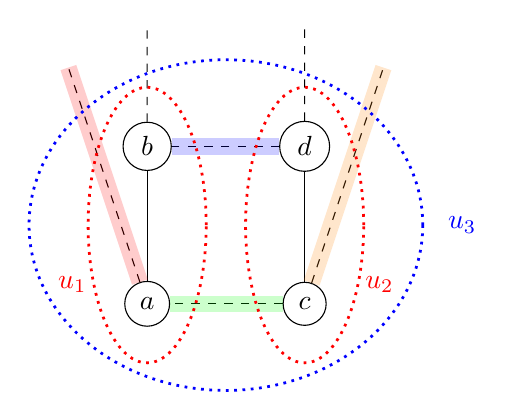
\begin{tikzpicture}
		\node [draw,circle] at (0,0) (a) {$a$};
		\node [draw,circle] at (0,2) (b) {$b$} edge (a);
		\node [draw,circle] at (2,0) (c) {$c$} edge [dashed] (a) edge [color=green,line width=6pt,opacity=0.2] (a) ;
		\node [draw,circle] at (2,2) (d) {$d$} edge (c) edge [dashed] (b) edge [line width=6pt,opacity=0.2,color=blue] (b);
		\draw [dashed] (a) -- +(-1,3)  (b) -- +(0,1.5) (d) -- +(0,1.5) (c) --  +(1,3);
		\draw [color=red,line width=6pt,opacity=0.2] (a) -- +(-1,3);
		\draw [color=orange,line width=6pt,opacity=0.2] (c) --  +(1,3);
		\draw [dotted,line width=1pt, color=red] (0,1) ellipse (0.75 and 1.75)
			(2,1) ellipse (0.75 and 1.75);
		\draw[line width=1pt,dotted,color=blue]	(1,1) ellipse (2.5 and 2.1);
		\node [color=red]at (-0.95,0.25) () {$u_1$};
		\node [color=red] at (2.95,0.25) () {$u_2$};
		\node [color=blue] at (4,1) () {$u_3$};
		
	\end{tikzpicture}
	\quad \quad \quad
	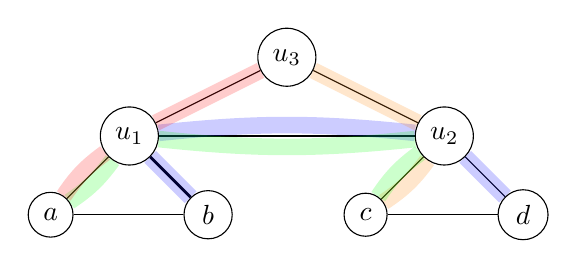
\begin{tikzpicture}
		\node [circle,draw] at (0,0) (a) {$a$};
		\node [circle,draw] at (2,0) (b) {$b$} edge (a);
		\node[circle,draw]  at (1,1) (u1) {$u_1$} edge (a) edge [color=green,opacity=0.2,line width=6pt,bend left=10] (a) edge [opacity=0.2,line width=6pt,color=red,bend right=10] (a) edge [line width=1pt](b) edge [color=blue,opacity=0.2,line width=6pt](b);
		\node[circle,draw]  at (4,0) (c) {$c$};
		\node [circle,draw] at (6,0) (d) {$d$} edge (c);
		\node [circle,draw] at (5,1) (u2) {$u_2$} edge (c) edge [color=orange,line width=6pt,opacity=0.2,bend left=10] (c) edge [color=green,opacity=0.2,line width=6pt,bend right=10] (c) edge (d) edge [color=blue,opacity=0.2,line width=6pt] (d) edge (u1) edge [color=blue,opacity=0.2,line width=6pt,bend right=6] (u1) edge [color=green,opacity=0.2,line width=6pt,bend left=6] (u1);
		\node[circle,draw]  at (3,2) (u3) {$u_3$} edge (u1) edge [color=red,opacity=0.2,line width=6pt] (u1) edge (u2) edge [color=orange,line width=6pt,opacity=0.2] (u2) ;
	\end{tikzpicture}
	\caption{An example of part of a hierarchy with three triangles. The graph on the left shows part of a feasible LP solution where dashed (and sometimes colored) edges have fraction $1/2$ and solid edges have fraction 1. The dotted ellipses on the left show the min-cuts $u_1,u_2,u_3$ in the graph. (Each vertex is also a min-cut). On the right is a representation of the corresponding hierarchy. Triangle $u_1$ corresponds to the cut $\{a,b\}$, $u_2$ corresponds to $\{c,d\}$ and $u_3$ corresponds to $\{a,b,c,d\}$. Note that, for example, the edge $(a,c)$, represented in green,  is in $\delta(u_1)$,  $\delta(u_3)$, and inside $u_3$.  For triangle $u_1$, we have $A=\delta(a)\smallsetminus (a,b)$ and $B = \delta(b)\smallsetminus (b,d)$.}
	\label{fig:hierarchywithtriangle}
\end{figure}
We will refer to the set of edges $E(X, \overline{S})$  (resp. $E(Y, \overline{S})$) as $A$ (respectively $B$) for a triangle cut $S$.  In addition, we say a triangle cut $S$ is {\em happy} if $A_T$ and $B_T$ are both odd. All non-triangle cuts are called degree cuts. A degree cut $S$ is {\em happy} if $\delta(S)_T$ is even.

\begin{theorem}[Main Payment Theorem (informal)]\label{thm:paymentinformal}
Let \hyperlink{tar:G=(V,E,x)}{$G=(V,E,x)$} for LP solution $x$ and let $\mu$ be the max-entropy distribution with marginals $x$ and $\decrease > 0$.
Given a hierarchy $\cH$, there is a slack vector $s: E\rightarrow \R$  such that
\begin{enumerate}[i)]
\item 	For each edge $e \in E$, $s_e \ge -x_e \decrease$. 
\item
For each cut $S\in \cH$  if $S$ is not happy, then $s(\delta(S))  \ge  0.$
\item For every LP edge $e\neq e_0$, $\E{s_e}\leq -\beta \eps_P x_e$ for  $\eps_P>0$.
\end{enumerate}

\end{theorem}




%As discussed above, consider an initial  O-join solution in which  $y_e := z_e/2$ for each edge $e$. We will modify this initial solution using the {\em slack vectors} $s$ and $s^*$ (which are initialized to 0). The first
% part of the proof shows that we can restrict attention to constructing a slack vector $s$ for a {\em subset} of the near-min-cuts that form a {\em hierarchy} $\cH$ --  a laminar family of near-min-cuts.
%  
% To ensure that those cuts that are {\em not} included in the hierarchy are satisfied in the final O-join solution, we will increase the slack $s^*(e^*)$ on some OPT edges $e^* \in E^*$.  
%
%
%The proof of this theorem has two main components.
In the following subsection, we discuss how to prove this theorem. Here we explain at a high level how to define the hierarchy and reduce \cref{thm:maintechnical} to this theorem. The details are in \cref{sec:polygons}.

First, observe that, given \cref{thm:paymentinformal}, cuts in $\cH$ will automatically satisfy (ii) of \cref{thm:maintechnical}. The approach we take to satisfying 
all other cuts is to introduce additional slack, the vector $s^*$, on $OPT$ edges. 

Consider the set of all near-min-cuts of $z$, where $z := (x + OPT)/2$.  Starting with $z$ rather than $x$ allows us to restrict attention to a significantly {\em more structured} collection of near-min-cuts. The key observation here is that in $OPT$, all min-cuts have value 2, and any non-min-cut has value {\em at least} 4. Therefore averaging  $x$ with $OPT$ guarantees that every $\eta$-near min-cut of $z$  must consist of a {\em contiguous sequence of vertices (an interval) along the OPT cycle}. Moreover, each of these cuts is a $2\eta$-near min-cut of $x$.  Arranging the vertices in the $OPT$ cycle around a circle, we identify every such cut with the interval of vertices that does not contain $(u_0, v_0)$. Also, we say that a cut is crossed on both sides if it is crossed on the left and on the right.



To ensure that any cut $S$ that is {\em crossed on both sides} is satisfied, we first observe that $S$ is odd with probability  $O(\eta)$.  To see this, let $S_L$ and $S_R$ be the cuts crossing $S$ on the left and right with minimum intersection with $S$ and consider
the two (bad) events $\{E(S\cap S_L, S_L \smallsetminus S))_T\ne 1\}$
and $\{E(S\cap S_R, S_R \smallsetminus S))_T\ne 1\}$. Recall that if $A,B$ and $A\cup B$ are all near-min-cuts, then $\P{ E(A,B)_T \ne  1}=  O(\eta)$ (see \cref{lem:treeoneedge}).
Applying this fact to the two aforementioned bad events implies that each of them has probability $O(\eta)$. Therefore, we will let the two $OPT$ edges in $\delta(S)$ be responsible for these two events, i.e.,   we will increase the slack $s^*$ on these two $OPT$ edges by $O(\eta)$ when the respective bad events happens. This gives  $\E{s^*(e^*)} = O(\eta^2)$ for each OPT edge $e^*$. As we will see, this  simple step will reduce the number of near-min-cuts of $z$ that we need to worry about satisfying to $O(n)$.


Next, we consider the set of near-min-cuts of $z$ that are crossed on at most one side. Partition these into maximal connected components of crossing cuts. Each such component corresponds to an interval along the OPT cycle and, by definition, these intervals form a laminar family. 

A single connected component $\cC$ of at least two crossing cuts  is called a {\em polygon}. 
We prove the following structural theorem about the polygons induced by $z$:

\begin{theorem}[Polygons look like cycles (Informal version of \cref{thm:poly-structure})]\label{thm:approxpoly}
Given a connected component $\cC$ of near-min-cuts of $z$ that are crossed on one side, consider the coarsest partition of vertices of the OPT cycle into 
a sequence  $a_1, \ldots, a_{m-1}$ of sets called atoms (together with $a_0$ which is the set of vertices not contained in any cut of $\cC$). Then 
\begin{itemize}
\item Every cut in $\cC$ is the union of some number of consecutive atoms in $a_1, \ldots, a_{m-1}$.
\item 	For each $i$ such that  $0\le i < m-1$, $x(E(a_i, a_{i+1})) \approx 1$ and similarly $x(E(a_{m-1}, a_{0})) \approx 1$.
\item For each $i>0$, $x(\delta(a_i))\approx 2$.
\end{itemize}
 
\end{theorem}


The main observation used to prove \cref{thm:approxpoly} is that the cuts in $\cC$ crossed on one side can be partitioned into two laminar families $\cL$ and $\cR$, where $\cL$ (resp. $\cR$) is the set of cuts crossed on the left (resp. right).
This immediately implies that $|\cC|$ is linear in $m$. Since cuts in $\cL$ cannot cross each other (and similarly for $\cR$), the proof boils down to understanding the interaction between $\cL$ and $\cR$.

The approximations in \cref{thm:approxpoly} are correct up to $O(\eta)$. Using additional slack in $OPT$, at the cost of an additional $O(\eta^2)$ for edge, we can treat these  approximate equations as if they are exact. Observe that if $x(E(a_i, a_{i+1})) =1$, and $x(\delta(a_i))=x(\delta(a_{i+1}))=2$
for $1 \le i \le m-2$, then with probability 1, $E(a_i, a_{i+1})_T = 1$. Therefore, any cut in $\cC$ which doesn't include $a_1$ or $a_{m-1}$ is even with probability 1. The  cuts in $\cC$ that contain $a_1$ are even precisely\footnote{Roughly, this corresponds to the definition of the polygon being left-happy.} when $E(a_0, a_1)_T$ is odd and similarly the cuts in $\cC$ that contain $a_{m-1}$ are even when $E(a_0, a_{m-1})_T$ is odd. These observations are what allow us to imagine that each polygon is a triangle, i.e., assume $m=3$. (Note that often it is convenient to look at the event in which $E(a_0, a_1)_T = 1$ and $E(a_0, a_{m-1})_T = 1$ since this is a simple criteria which implies that all cuts in $\cC$ are even.)

The hierarchy $\cH$ is the set of all $\eta$-near mincuts of $z$ that are not crossed at all (these will be the degree cuts), together with a triangle for every polygon. In particular, for a connected component $\cC$ of size more than 1, the corresponding triangle cut is $a_1\cup \ldots \cup a_{m-1}$, with $A = E(a_0, a_1)$ and $B = E(a_0, a_{m-1})$. Observe that from the discussion above, when a triangle cut is happy, then all of the cuts in the corresponding polygon $\cC$ are even.
 
 
 Summarizing, we show that if we can construct a good slack vector $s$ for a hierarchy of degree cuts and triangles, then there is a nonnegative slack vector $s^*$, that satisfies all near-minimum cuts of $z$ not represented in the hierarchy, while maintaining slack for each OPT edge $e^*$ such that $\E{s^*(e^*)} = O(\eta^2)$. 
 
 
 \paragraph{Remarks:}
 
 The reduction that we sketched above only uses the fact that $\mu$ is an arbitrary distribution of spanning trees with marginals $x$ and not necessarily a maximum-entropy distribution.
 
 We also observe that to prove \cref{thm:main}, we crucially used that $28 \eta \ll \eps$.  This forces us to take $\eta$ very small, which is why we get only a ``very slightly'' improved approximation algorithm for TSP. Furthermore, since we use OPT edges in our construction, we don't get a new upper bound on the integrality gap.  We leave it as an open problem to find a reduction to the ``cactus'' case that doesn't involve using a slack vector for OPT (or a completely different approach).

 
 
 \subsection{Proof ideas for \cref{thm:paymentinformal}}
 
 We now address the problem of constructing a good slack vector $s$ for a hierarchy of degree cuts and triangle cuts.
 For each LP edge $f$, consider the lowest cut in the hierarchy, that contains both endpoints of $f$. We call this cut $\p(f)$.
 If $\p(f)$ is a degree cut, then we call $f$ a {\em top edge} and otherwise, it is a {\em bottom edge}\footnote{For example, in \cref{fig:hierarchywithtriangle}, $\p(a,c) = u_3$, and $(a,c)$ is a bottom edge.}. We will see that bottom edges are easier to deal with, so we start by discussing the slack vector $s$ for top edges.
  
 Let $S$ be a degree cut and let $\bbe = (u,v)$ (where $u$ and $v$ are children of $S$ in $\cH$) be the set of all top edges $f = (u', v')$ such that $u' \in u$ and $v' \in v$. We call $\bbe$ a {\em top edge bundle} and say that $u$ and $v$ are the {\em top cuts} of each $f \in \bbe$. We will also sometimes say that $\bbe \in S$.
 
 Ideally, our plan is to reduce the slack of every edge $f \in \bbe$ when it is {\em happy}, that is, both of its top cuts are even in $T$. Specifically, we will set  $s_f := -\eta x_f$ when  $\delta(u)_T$ and $ \delta(v)_T $ are even. When this happens, we say that $f$ is {\em reduced}, and refer to the event $\{\delta(u)_T,\delta(v)_T\text{ even}\}$ as the {\em reduction event} for $f$.
 Since this latter event doesn't depend on the actual endpoints of $f$, we view this as a simultaneous reduction of $s_\bbe$. 
 
Now consider the situation from the perspective of the degree cut $u$ (where $\p(u)=S$) and consider any incident edge bundle in $S$, e.g., $\bbe = (u,v)$. Either its top cuts are both even and $s_\bbe := - \eta x_\bbe$, or they aren't even, because, for example, $\delta(u)_T$ is odd. In this latter situation,  edges in   $\delta^\uparrow(u):= \delta(u)\cap \delta(S)$ might have been reduced (because {\em their} top two cuts are even), which a priori could leave $\delta(u)$ \hyperlink{tar:satisfy}{unsatisfied}. In such a case, we {\em increase} $s_\bbe$ for edge bundles in $ \delta^\rightarrow(u):= \delta (u) \smallsetminus \delta(S)$ to compensate for this reduction.  Our main goal is then to prove is that for any edge bundle its expected reduction is greater than its expected increase.
  The next example shows this analysis in an ideal setting. 

 
 
\begin{example}[Simple case] \label{ex:simple}
Fix a top edge bundle $\bbe = (u,v)$ with $\p(\bbe) = S$.
Let $x_u := x(\delta^\uparrow (u))$ and let $x_v := x(\delta^\uparrow (v))$. Suppose we have constructed a (fractional) {\em matching} between edges whose top two cuts are children of $S$ in $\cH$ and the edges in $\delta(S)$, and this matching satisfies the following three conditions: (a) $\bbe=(u,v)\in S$ is matched (only) to edges going higher from its top two cuts (i.e., to edges in $\delta^\uparrow (u)$ and $\delta^\uparrow (v)$),  (b) $\bbe$ is matched to  
an $m_{\bbe,u}$ fraction of every edge in $\delta^\uparrow(u)$ and to an $m_{\bbe,v}$ fraction of each edge in $\delta^\uparrow(v)$, where
$$m_{\bbe,u}  + m_{\bbe, v}  = x_\bbe,$$ and (c) the fractional value of edges in $\delta^\rightarrow(u):= \delta(u) \smallsetminus \delta^\uparrow(u)$ matched to edges in $\delta^\uparrow(u)$  is equal to $x_u$. That is, for each $u\in S$, $\sum_{\bbf \in \delta^\rightarrow(u)} m_{\bbf,u} = x_u$.

\begin{figure}[htb]
\centering	
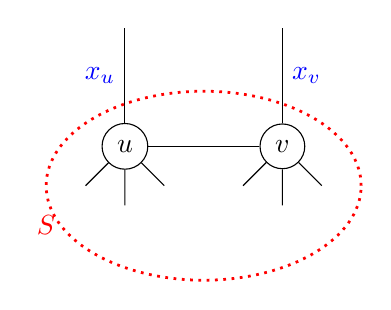
\begin{tikzpicture}
	\node [circle,draw] at (0,0) (u) {$u$};
	\node [circle,draw] at (2,0) (v) {$v$} edge node [above] {$\bbe$} (u);
	\draw (u) -- node [left] {\color{blue}{$x_u$}} +(0,1.5) (v) -- node [right] {\color{blue}{$x_v$}} +(0,1.5);
	\draw [dotted,color=red,line width=1pt] (1,-0.5) ellipse (2 and 1.2) ;
	\draw (u) -- +(-0.5,-0.5) (v) -- +(-0.5,-0.5) (u) -- +(0.5,-0.5) (v) -- +(0.5,-0.5) (u) -- +(0,-0.75) (v) -- +(0,-0.75);
	%\draw [dotted,line width=4pt] (-0.25,-1) -- +(1.5,0);
	%\node [fill,circle,inner sep=4] at (0,-1) () {};
	%\node [fill,circle,inner sep=3] at (1,-1) () {};
	%\node [fill,circle,inner sep=5] at (2,-1) () {};
	\node [color=red] at (-1,-1) () {$S$};
\end{tikzpicture}
\end{figure}


The plan is for $\bbe\in S$ to be tasked with part of the responsibility for {\em fixing the cuts} $\delta(u)$ and $\delta(v)$ when they are odd and edges going higher are reduced. Specifically, $s_\bbe$ is increased to compensate for an $m_{\bbe,u}$  fraction of the reductions in edges in $\delta^\uparrow(u)$ when $\delta(u)_T$ is odd. (And similarly for reductions in $v$.) 
Thus,
%Suppose also that  $\P{\delta(u)_T = \delta(v)_T = 2 } = p$. 
%Let $E_u$ (resp. $E_v$) denote the set of edges in $\delta^\uparrow (u)$ (resp. $\delta^\uparrow(v)$) that $\bbe$ is matched to. Then we have
\begin{align}
	\E{s_\bbe} &= -\P{\bbe\text{ reduced}} \eta x_\bbe + m_{\bbe,u}\sum_{g\in \delta^\uparrow(u)} \P{\delta(u)_T\text{ odd}|g \text{ reduced} }\P{g \text{ reduced}}\eta \frac{x_g}{x(\delta^\uparrow(u))}\notag\\
	&\quad\quad +  m_{\bbe,v}\sum_{g\in \delta^\uparrow(v)} \P{\delta(v)_T\text{ odd}|g \text{ reduced} }\P{g \text{ reduced}}\eta \frac{x_g}{x(\delta^\uparrow(v))} \label{eq:sfUB}
\end{align}
We will lower bound  $\P{\delta(u)_T\text{ even}|g\text{ reduced}}$. We can write this as
$$\P{\delta^\rightarrow (u)_T\text{ and }\delta^\uparrow (u)_T\text{ have same parity } | g \text{ reduced}}.$$
Unfortunately, we do not currently have a  good handle on the parity of $\delta^\uparrow (u)_T$ conditioned on $g$ reduced. 
However,  we can use 
the following simple but crucial property: Since $x(\delta(S)) = 2$, by \cref{lem:treeconditioning}, $T$ consists of two independent trees, one on $S$ and one on $V \smallsetminus S$, each with the corresponding marginals of $x$.
Therefore, we can write$$\P{\delta(u)_T\text{ even}|g\text{ reduced}} \ge \min (\P{(\delta^\rightarrow (u))_T \text{ even}}, \P{(\delta^\rightarrow (u))_T \text{ odd}}).$$
This gives us a reasonable bound when $\eps \le x_u, x_v \le 1- \eps$ since, because
$x(\delta(u)) = x(\delta(v))=2$, 
by the SR property, $(\delta^\rightarrow (u))_T$ (and similarly $(\delta^\rightarrow (v))_T$) is the sum of Bernoulis with expectation in $[1+\eps, 2-\eps]$. From this it follows that 
$$ \min (\P{(\delta^\rightarrow (u))_T \text{ even}}, \P{(\delta^\rightarrow (u))_T \text{ odd}}) =\Omega (\epsilon). $$We can therefore conclude that 
$\P{\delta(u)_T\text{ odd}|g\text{ reduced}}  \le 1- O(\eps).$

The rest of the analysis of this special case follows  from (a) the fact that our construction will guarantee that for {\em all} edges $g$, the probability that $g$ is reduced is {\em exactly} $p$, i.e., it is the same for all edges, and 
(b) the fact that $m_{\bbe,u}x_u + m_{\bbe,v}x_v = x_\bbe$.
Plugging these facts back into \eqref{eq:sfUB}, gives
\begin{align}
\E{s_\bbe} &\le  -p \eta x_\bbe + m_{\bbe,u} (1-\eps) p \eta  + 
m_{\bbe,v} (1-\eps) p \eta \notag\\
& \le -p\eta x_\bbe + (1-\eps)p\eta x_\bbe =
 -\eps p\eta x_\bbe.	\label{eq:sbbe}
\end{align}
If we could prove \eqref{eq:sbbe} for {\em every} edge $f$ in the support of $x$, that would complete the proof that the expected cost of the min $O$-join for a random spanning tree $T\sim\mu$ is at most $(1/2 - \eps) OPT$.
\end{example}

\paragraph{Remark:} 
Throughout this paper, we repeatedly use a mild generalization of the above "independent trees fact": that if $S$ is a cut with $x(\delta(S)) \le 2 + \eps$, then $S_T$ is very likely to be a tree. Conditioned on this fact, marginals inside $S$ and outside $S$ are nearly preserved and the trees inside $S$ and outside $S$ are sampled independently (see \cref{lem:treeconditioning}).

\paragraph{Ideal reduction:}
In the example, we were able to show that $\P{\delta(u)_T \text{ odd} \mid g\text{ reduced}}$ was bounded away from 1 for every edge $g\in \delta^\uparrow(u)$, and this is how we proved that the expected reduction for each edge was greater than the expected increase on each edge, yielding negative expected slack. 

This motivates the following definition: A reduction for an edge $g$ is $k$-{\em ideal}
 if, conditioned on $g$ reduced, every cut $S$ that is in the top $k$ levels of cuts containing $g$  is odd with probability that is bounded away from 1. 


\paragraph{Moving away from an idealized setting:}
In \cref{ex:simple}, we oversimplified in four ways:
\begin{enumerate}[(a)]
\item We assumed that it would be possible to show that each top edge is {\em good}. That is, that its top two cuts are even {\em simultaneously} with constant probability.

\item We considered only top edge bundles (i.e., edges whose top cuts were inside a degree cut).

\item 	We assumed that $x_u, x_v \in [\epsilon, 1-\epsilon]$.
\item We assumed the existence of a nice matching between edges  whose top two cuts were children of $S$ and the edges in $\delta(S)$.
\end{enumerate}
Our proof needs to address all four anomalies that result from deviating from these assumptions. 

\begin{figure}[htb]\centering
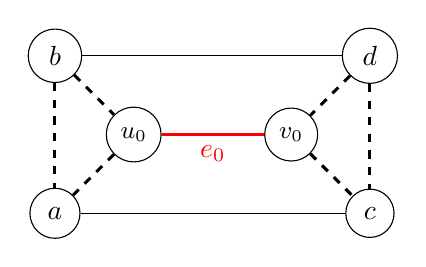
\begin{tikzpicture}
	\node [draw,circle,inner sep=4] at (0,0) (a)  {$a$};
	\node [draw,circle] at (1,1) (b)  {{\small$u_0$}}  edge [dashed, line width=1.1pt] (a);
	\node [draw,circle,inner sep=4] at (0,2) (c)  {$b$}  edge [dashed, line width=1.1pt] (b) edge [dashed, line width=1.1pt] (a);
	
	\node [draw,circle,inner sep=4] at (4,0) (d)  {$c$} edge  (a);
	\node [draw,circle] at (3,1) (e)  {{\small$v_0$}}  edge [dashed, line width=1.1pt] (d) edge  [color=red,line width=1.1pt]  node [below] {$e_0$} (b);
	\node [draw,circle,inner sep=4] at (4,2) (f)  {$d$}  edge [dashed, line width=1.1pt] (d) edge [dashed, line width=1.1pt] (e) edge(c);
\end{tikzpicture}
\caption{An Example with Bad Edges. A feasible solution of the \ref{eq:tsplp} is shown; dashed edges have fraction 1/2 and solid edges have fraction 1. Writing $E=E_0\smallsetminus \{e_0\}$ as a maximum entropy distribution $\mu$ we get the following: Edges $(a,b),(c,d)$ must be completely negatively correlated (and independent of all other edges). So, $(b,u_0), (a,u_0)$ are also completely negatively correlated. This implies $(a,b)$ is a bad edge. }
\label{fig:badedgeexistence}
\end{figure}

\paragraph{Bad edges.} Consider first (a). Unfortunately, it is not the case that all top edges are good. Indeed, some are {\em bad}.  However, it turns out that bad edges are rare in the following senses: First, for an edge  to be bad, it must be a half edge, where we say that an edge $\bbe$ is a half edge if  $x_\bbe \in 1/2 \pm \eps_{1/2}$ for a suitably chosen constant $\eps_{1/2}$. Second, of any two half edge bundles sharing a common endpoint in the hierarchy, at least one is good. For example, in \cref{fig:badedgeexistence}, $(a,u_0)$ and $(b,u_0)$ are good half-edge bundles. We advise the reader to ignore half edges in the first reading of the paper. Correspondingly, we note that our proofs would be much simpler if half-edge bundles never showed up in the hierarchy. It may not be a coincidence that half edges are hard to deal with, as it is conjectured that TSP instances with half-integral LP solutions are the hardest to round~\cite{SWV12,SWvZ13}.

Our solution is to {\em never} reduce bad edges. But this in turn poses two problems. First, it means that we need to address the possibility that the bad edges constitute most of the cost of the LP solution. Second, our objective is to get negative expected slack on each good edge and non-positive expected slack on bad edges. Therefore, if we never reduce bad edges, we can't increase them either, which means that the responsibility for fixing an odd cut with reduced edges going higher will have to be split amongst fewer edges (the incident good ones). 


We deal with the first problem by showing that 
in every cut $u$ in the hierarchy at least 3/4 of the fractional mass in $\delta(u)$ is good and these edges suffice to compensate for reductions on the edges going higher. Moreover, because  there are sufficiently many good edges incident to each cut, we can show that either using the slack vector $\{s_e\}$ gives us a low-cost O-join, or we can average it out with another O-join solution concentrated on bad edges to obtain a reduced cost matching of odd degree vertices.

We deal with the second problem by proving \cref{lem:matching}, which guarantees a matching between  {\em good} edge bundles $\bbe = (u,v)$ and fractions $m_{\bbe,u}, m_{\bbe,v}$ of edges in $\delta^\uparrow(u), \delta^\uparrow(v)$ such that, roughly, $m_{\bbe,u} + m_{\bbe,v} = (1 + O(\eps_{1/2}))x_\bbe$. 


\paragraph{Dealing with triangles.} \hypertarget{211-explanation}{Turning to (b)}, consider  a triangle cut $S$, for example $\delta(a_1 \cup a_2)$ in \cref{fig:twotriangles}.
Recall that in a triangle, we can assume that there is an edge of fractional value 1 connecting $a_1$ and $a_2$ in the tree, and this is why we defined the cut to be happy when $A_T$ and $B_T$ are odd: this guarantees that all 3 cuts  defined by the triangle ($\delta(a_1),\delta(a_2), \delta(a_1 \cup a_2)$ are even. %(For further details see \cref{fig:twotriangles}.)

\begin{figure}\centering
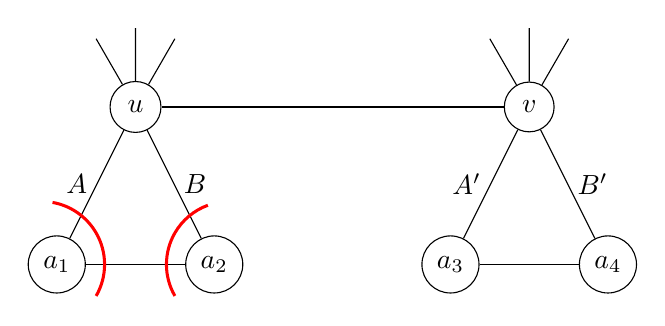
\begin{tikzpicture}
	\node [draw,circle] at (0,0) (a1) {$a_1$};
	\node [draw,circle] at (2,0) (a2) {$a_2$} edge node [below] {$\bbf$} (a1) ;
	\node [draw,circle,inner sep=4] at (1,2) (u) {$u$} edge node [left] {$A$} (a1) edge node [right] {$B$} (a2) ;
	\node [draw,circle] at (5,0) (a3) {$a_3$};
	\node [draw,circle] at (7,0) (a4) {$a_4$} edge node [below] {${\bbg}$} (a3);
	\node [draw,circle,inner sep=4] at (6,2) (v) {$v$} edge node [above] {$\bbe$} (u) edge node [left] {$A'$} (a3) edge node [right] {$B'$} (a4);
	\draw [color=red, line width=1.1pt](0.5,-0.4) arc (-30:80:0.8)
	(1.5,-0.4) arc (210:110:0.8);
	\draw (u) -- +(60:1) (u) -- +(90:1) (u) -- +(120:1) (v) -- +(60:1) (v) -- +(90:1) (v) -- +(120:1);;
\end{tikzpicture}
\caption{In this representation of the cut hierarchy (as in \cref{fig:hierarchywithtriangle}), for the triangle $u$ corresponding to the cut $\delta(a_1\cup a_2)$, when $A_T$ and $B_T$ are odd, all 3 cuts ($\delta(a_1)_T, \delta(a_2)_T$ and $\delta(a_1 \cup a_2)_T = \delta(u)_T$ are odd (since $\bbf_T$ is always 1). (Recall also that the edges in the bundle $\bbe$ must have one endpoint in $\{a_1 \cup a_2\}$ and one endpoint in $\{a_3 \cup a_4\}$, as was the case, e.g., for the edge $(a,c)$ in \cref{fig:hierarchywithtriangle}.)}
\label{fig:twotriangles}
\end{figure}
Now suppose that $\bbe = (u,v)$ is a top edge bundle, where $u$ and $v$ are both triangles, as shown in \cref{fig:twotriangles}. Then we'd like to reduce $s_\bbe$ when both cuts $u$ and $v$ are happy. But this would require more than simply both cuts being even. This would require  {\em all} of 
$A_T, B_T, A'_T, B'_T$ to  be odd. Note that if, for whatever reason,  $\bbe$ is reduced only when $\delta(u)_T$ and $\delta(v)_T$ are both even, then it could be, for example, that this only happens when $A_T$ and $B_T$ are both even. In this case, both $\delta(a_1)_T$ and $\delta(a_2)_T$ will be odd with probability 1 (recalling that $\bbf_T=1$), which would then necessitate an increase in $s_\bbf$ whenever $\bbe$ is reduced. In other words, the reduction will not even be 1-ideal.


It turns out to be easier for us to get a 1-ideal reduction rule for $\bbe$ as follows: Say that
$\bbe$ is {\em 2-1-1 happy with respect to $u$} if  $\delta(u)_T$ is even and both $A'_T, B'_T$ are odd. We reduce $\bbe$ with probability $p/2$ when it is 2-1-1 happy with respect to $u$ and with probability $p/2$ when it is 2-1-1 happy with respect to $v$. This means that when $\bbe$ is reduced, half of the time no increase in $s_\bbf$ is needed since $u$ is happy. Similarly for $v$. 
 

The 2-1-1 criterion for reduction introduces a new kind of bad edge: a half edge that is good, but not 2-1-1 good. We are able to show that non-half-edge bundles are 2-1-1 good (\cref{lem:x_e<=1/2-eps1,lem:x_e>=1/2+eps_1/2}), and that if there are two half edges which are both in $A$ or are both in $B$, then at least one of them is 2-1-1 good (\cref{lem:one-of-two-211}). Finally, we show that if there are two half edges, where one is in  $A$ and the other is in $B$, and neither is 2-1-1 good, then we can apply a different reduction criterion that we call {\em 2-2-2 good}. When the latter applies, we are guaranteed to decrease both of the half edge bundles simultaneously.
All together, the various considerations discussed in this paragraph force us to come up with a relatively more complicated set of rules under which we reduce $s_\bbe$ for a top edge bundle $\bbe$ whose children are triangle cuts. \cref{sec:probabilistic} focuses on developing the relevant probabilistic statements.


\paragraph{Bottom edge reduction.} Next, consider a bottom edge bundle $\bbf = (a_1,a_2)$ where $\p(a_1) = \p(a_2)$ is a triangle. Our plan is to reduce $s_\bbf$ (i.e., set it to $-\eta x_\bbf$) when the triangle is happy, that is, $A_T = B_T = 1$. The good news here is that every triangle is happy with constant probability. However, when a triangle is {\em not} happy, $s_\bbf$ may need to increase to make sure that the O-join constraint for $\delta(a_1)$ and $\delta(a_2)$  are satisfied, if
 edges in $A$ and $B$ going higher are reduced. Since  $x_\bbf = x(A) = x(B) = 1$, this means that $\bbf$ may need to compensate at {\em twice} the rate at which it is getting reduced. This would result in $\E{s_\bbf}>0$, which is the opposite of what we seek.
 
 We use two key ideas to address this problem.  First, we reduce top edges and bottom edges by different amounts: Specifically, when the relevant reduction event occurs, we reduce a bottom edge $\bbf$  by $\beta x_\bbf$ and top edges $\bbe$ by $\tau x_\bbe$, where $\beta >   \tau$ (and $\tau$ is a multiple of $\eta$). 

Thus, the expected reduction in $s_\bbf$ is $p\beta x_\bbf = p\beta$, whereas the expected increase (due to compensation of, say, top edges going higher) is $p\tau (x(A) + x(B))q = p \tau 2 q$,
where $$q = \P{\text{ triangle not happy} \mid \text{reductions in $A$ and $B$}}.$$ Thus, so long as $2 \tau q < \beta - \epsilon$, we get the expected reduction in $s_\bbf$ that we seek.

The discussion so far suggests that we need to take $\tau$ smaller than $\beta/2q$, which is $\beta/2$ if $q$ is 1, for example. On the other hand, if $\tau = \beta/2$, then when a top edge needs to fix a cut due to reductions on bottom edges, we have the opposite problem -- their expected increase will be greater than their expected reduction, and we are back to square one.

Coming to our aid is the second key idea, already discussed in \cref{sec:marginals}.  We reduce bottom edges only when $A_T = B_T = 1$ {\em and} the marginals of edges in $A,B$ are approximately preserved (conditioned on $A_T = B_T = 1$). This allows us to get much stronger upper bounds on the probability that a lower cut a bottom edge is on is odd, given that the bottom edge is reduced, and enables us to show that bottom edge reduction is $\infty$-ideal.

It turns out that the combined effects of (a) choosing $\tau =0.571 \beta$, and (b) getting better bounds on the probability that a lower cut is even given that a bottom edge is reduced, suffice to deal with the interaction between the reductions and the increases in slack for top and bottom edges.


\begin{figure}[htb]\centering
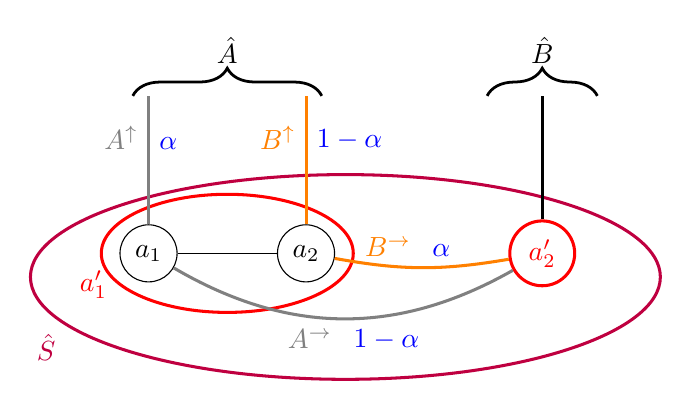
\begin{tikzpicture}
\node [draw,circle]at (0,0) (a1) {$a_1$} ;
\node [draw,circle] at (2,0) (a2) {$a_2$} edge node [below] {$\bbf$} (a1);
\draw [color=red,line width=1.1pt] (1,0) ellipse  (1.6 and 0.75);
\draw [line width=1.1pt,color=purple] (2.5,-0.3) ellipse (4 and 1.3);
\node [color=purple] at (-1.3,-1.2) () {$\hat{S}$};
\draw [line width=1pt, decorate,decoration={brace,amplitude=10pt}]
(-0.2,2) -- node [above=8] {$\hat{A}$} (2.2,2);
\draw [line width=1pt, decorate,decoration={brace,amplitude=10pt}]
(4.3,2) -- node [above=8] {$\hat{B}$} (5.7,2);

\node [color=red,line width=1.1pt] at (-0.7,-0.4)  () {$a_1'$};
\node [color=red,draw,circle,line width=1.1pt] at (5,0) (a3) {$a_2'$} edge [color=gray,bend left=30,line width=1.1pt] node [below left] {$A^\rightarrow$} node [below right,color=blue] {\textcolor{blue}{$1-\alpha$}} (a1) edge [color=orange, line width=1.1pt,bend left=10] node [above left] {$B^\rightarrow$} node [above right,color=blue] {\textcolor{blue}{$\alpha$}} (a2);
\draw [line width=1.1pt,color=gray] (a1) -- node [above left]{$A^\uparrow$} node [above right, color=blue ] {\textcolor{blue}{$\alpha$}} +(0,2);
\draw [line width=1.1pt,color=orange] (a2) -- node [above left]{$B^\uparrow$} node [above right,color=blue] {\textcolor{blue}{$1-\alpha$}} +(0,2);
\draw [line width=1.1pt] (a3) --  +(0,2);
\end{tikzpicture}	
\caption{Setting of \cref{ex:bottombottom}. Note that the set $A = \delta(a_1) \cap \delta(a_1')$  decomposes into two sets of edges, $A^\uparrow$, those that are also in $\delta(S)$, and the rest, which we call $A^\rightarrow$. Similarly for $B$.}
\label{fig:bottombottom}
\end{figure}

\begin{example}\label{ex:bottombottom} [Bottom-bottom case]
To see how preserving marginals helps us handle the interaction between bottom edges at consecutive levels, consider a triangle cut $a_1' = \{a_1, a_2\}$ whose parent cut $\hat{S} = \{a_1', a_2'\}$ is also a triangle cut (as shown in \cref{fig:bottombottom}). 
Let's analyze $\E{s_\bbf}$ where $\bbf = (a_1, a_2)$. Observe first that
$A^\rightarrow\cup B^\rightarrow$ is a bottom edge bundle in the triangle $\hat S$ and all edges in this bundle are reduced simultaneously when $\hat{A}_T = \hat{B}_T = 1$
and marginals of all edges in $\hat{A}\cup\hat{B}$ are approximately preserved. (For the purposes of this overview, we'll assume they are preserved exactly). Furthermore, since the tree inside $\hat{S}$ is picked independently of the tree on $G/\hat{S}$ (using \cref{lem:treeconditioning} and assuming $\epsilon = 0$ for this overview), exactly one edge in $A^\rightarrow\cup B^\rightarrow$ is selected independently of the reduction event $\hat{A}_T = \hat{B}_T = 1$. Let $x(A^\uparrow) = \alpha$. Then since $A = A^\uparrow \cup A ^\rightarrow$ and $x(A)=1$, we have $x(A ^\rightarrow) = 1-\alpha$.
Moreover, since $\hat A = A^\uparrow \cup B^\uparrow$ and $x(\hat A)=1$, we also have
$x(B ^\uparrow) =1- \alpha$ and  $x(B ^\rightarrow) = \alpha$.

Therefore, using the fact that when $A^\rightarrow \cup B^\rightarrow$ is reduced, exactly one edge in $A^\uparrow \cup B^\uparrow$ is selected (and also exactly one edge in $A^\rightarrow \cup B^\rightarrow$ is selected independently since it is a bottom edge bundle, as mentioned above),  and marginals are preserved given the reduction,
 we conclude that
$$\P{a_1'\text{ happy} \mid A^\rightarrow \cup B^\rightarrow\text{ reduced}}  =\P{A_T= B_T = 1 \mid A^\rightarrow \cup B^\rightarrow\text{ reduced}}  =\alpha^2 + (1-\alpha)^2. $$
Now, we calculate $\E{s_\bbf}$. First, note that $\bbf$ may have to increase to compensate either for reduced edges in $A^\uparrow\cup B\uparrow$ or in $A^\rightarrow\cup B
^\rightarrow$.
For the sake of this discussion, suppose that $A^\uparrow \cup B^\uparrow$ is a set of top edges. Then, in the worst case we need to increase $\bbf$ by $p\tau$ in expectation to fix the cuts $a_1,a_2$ due to the reduction in $A^\uparrow \cup B^\uparrow$.
Now, we calculate the expected increase due to the reduction in $A^\rightarrow\cup B^\rightarrow$.
The crucial observation is that edges in $A^\rightarrow \cup B^\rightarrow$ are reduced simultaneously, so both cuts $\delta(a_1)$ and $\delta(a_2)$ can be fixed simultaneously by an increase in $s_\bbf$. Therefore, when they are both odd,  it suffices for $\bbf$ to increase by 
$$\max\{x(A^\rightarrow), x(B^\rightarrow)\}\beta = \max \{\alpha, 1-\alpha\}\beta,$$ 
to fix cuts $a_1,a_2$. Putting this together, we get
\begin{align*}
	\E {s_\bbf} & = -p\beta + \E{\text{increase due to }A^\rightarrow \cup B^\rightarrow} + \E{\text{increase due to }A^\uparrow \cup B^\uparrow}\\
	&\le -p\beta  +p\beta \max_{\alpha \in [1/2, 1] }\alpha[1-\alpha^2 - (1-\alpha)^2] + p\tau\\
	\intertext{which, since  $\max_{\alpha \in [1/2, 1] }\alpha[1-\alpha^2 - (1-\alpha)^2]= 8/27$ and  $\tau = 0.571 \beta$ is}
	&= p\beta (-1 + \frac{8}{27} + 0.571) = -0.13 p \beta.
\end{align*}
\end{example}

\paragraph{Dealing with $x_u$ close to $1$.}\footnote{Some portions of this discussion might be easier to understand after reading the rest of the paper.} 
\hypertarget{ABC-explanation}{Now}, suppose that $\bbe=(u,v)$ is a top edge bundle with $x_u:=x(\delta^\uparrow(u))$ is close to  $1$.
 Then, the  analysis in \cref{ex:simple}, bounding $r:= \P{\delta(u)_T \text{ odd} | g\text{ reduced}}$ away from 1 for an edge $g\in \delta^\uparrow(u)$ doesn't hold.
To address this, we consider two cases:
The first case, is that the edges in $\delta^\uparrow(u)$ break up into many groups that end at different levels in the hierarchy.
In this case, we can analyze $r$ separately for the edges that end at any given level, taking advantage of the independence between the trees chosen at different levels of the hierarchy.

The second case is when nearly all of the edges in   $\delta^\uparrow(u)$ end at the same level, for example, they are all in $\delta^\rightarrow(u')$ where $\p(u')$ is a degree cut. In this case,
we introduce a more complex (2-1-1) reduction rule for these edges.
The observation is that from the perspective of these edges $u'$ is a "pseudo-triangle". That is, it looks like a triangle cut, with atoms $u$ and $u'\smallsetminus u$ where $\delta(u)\cap\delta(u')$ corresponds to the ``$A$''-side of the triangle. %where $A= \delta^\uparrow (u)$ and $B = \delta(u') \smallsetminus \delta(u)$ where $x(A)=x_u\approx 1$ and $x(B)=x(\delta(u'))-x_u\approx 1$. 

Now, we define this more complex 2-1-1 reduction rule: Consider a top edge $\bbf=(u',v')\in\delta^\rightarrow(u')$. So far, we only considered the following reduction rule for $\bbf$: If both $u',v'$ are degree cuts, $\bbf$ reduces when they are both even in the tree; otherwise if say $u'$ is a triangle cut, $\bbf$ reduces when it is 2-1-1 good w.r.t., $u'$ (and similarly for $v'$). 
But clearly these rules ignore the pseudo triangle.  The simplest adjustment is, if $u'$ is a pseudo triangle with partition $(u,u'\smallsetminus u)$, to require $\bbf$ to reduce when $A_T=B_T=1$ and $v'$ is happy. However, as stated, it is not clear that the sets $A$ and $B$ are well-defined. For example, $u'$ could be an actual triangle or there  could be multiple ways to see $u'$ as a pseudo triangle only one of which is $(u, u'\smallsetminus u)$. Our solution is to find the {\em smallest} disjoint pair of cuts $a,b\subset u'$ in the hierarchy such that $x(\delta(a)\cap\delta(u')),x(\delta(b)\cap\delta(u'))\geq 1-\eps_{1/1}$, where $\eps_{1/1}$ is a fixed universal constant, and then let $A=\delta(a)\cap\delta(u'), B=\delta(b)\cap\delta(u')$ and $C=\delta(u')\smallsetminus A\smallsetminus B$ (see \cref{fig:topedgeABCmotivation} for an example). Then, we say $\bbf$ is 2-1-1 happy w.r.t., $u'$ if $A_T=B_T=1$ and $C_T=0$.

\begin{figure}[htb]
\centering
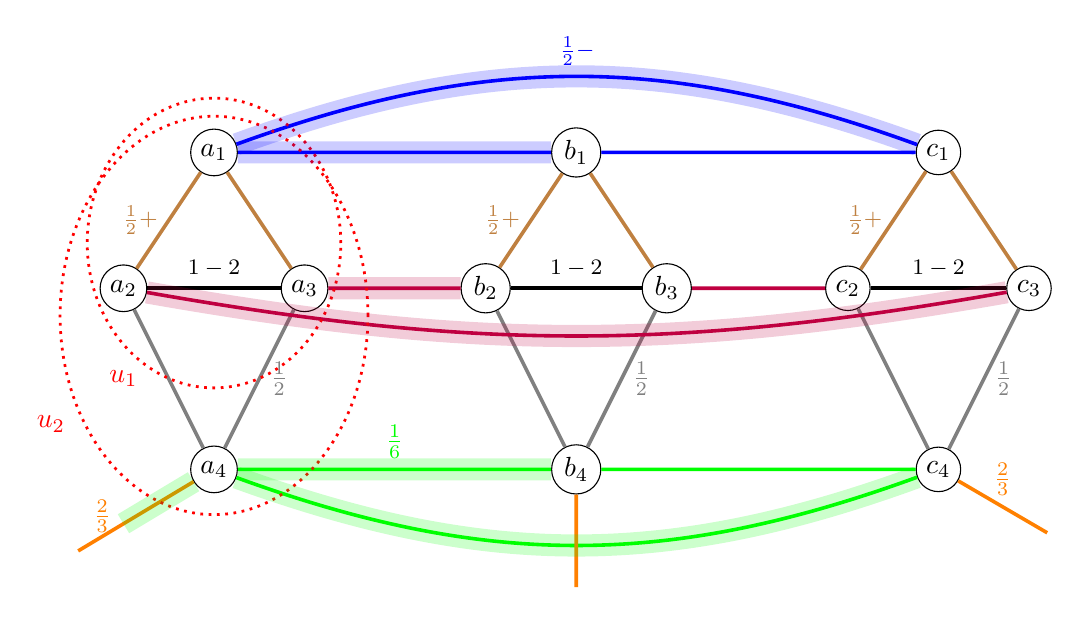
\begin{tikzpicture}[scale=1.15]
\foreach \i/\a in {0/a, 1/b, 2/c}{
	\node [draw,circle,inner sep=2] at (\i*4,2) (\a1) {$\a_1$};
	\node [draw,circle,inner sep=2] at (\i*4-1,0.5) (\a2) {$\a_2$} edge [color=brown,line width=1.3pt] node [left] {\footnotesize$\frac12+\eps$} (\a1);
	\node [draw,circle, inner sep=2] at (\i*4+1,0.5) (\a3) {$\a_3$} edge [color=brown,line width=1.3pt] (\a1) edge [line width=1.3pt] node [above] {\footnotesize{$1-2\eps$}} (\a2);
	\node [draw,circle, inner sep=2] at (\i*4, -1.5) (\a4) {$\a_4$} edge [line width=1.3pt,color=gray]  (\a2) edge [color=gray,line width=1.3pt] node [right] {$\frac12$} (\a3);
}
	\draw [color=green,line width=1.3pt] (a4) edge node [above] {$\frac16$} (b4) (b4) edge (c4) (c4) edge [bend left=20] (a4);
	\draw [color=orange,line width=1.3pt] (a4) -- node [left=5] {$\frac23$} +(-1.5,-0.9) (b4) --  +(0,-1.3)  (c4) -- node [above] {$\frac23$} +(1.2,-0.7);
	\draw [color=blue,line width=1.3pt] (a1) edge  (b1) (b1) edge (c1) (c1) edge [bend right=20] node [above] {\footnotesize$\frac12-\eps$} (a1);
	\draw [color=purple,line width=1.3pt] (a3) edge (b2) (b3) edge (c2) (c3) edge [bend left=10] node [below] {\footnotesize$\eps$} (a2);
	\draw [dotted,color=red,line width=1pt](0,1) ellipse (1.4 and 1.6)
	(0,0.2) ellipse (1.7 and 2.2);
	\node [color=red]at (-1.8,-1) () {$u_2$};
	\node [color=red] at (-1,-0.5) () {$u_1$};
	\draw [color=blue,line width=8pt,opacity=0.2] (a1) edge (b1)
	(a1) edge [bend left=20] (c1);
	\draw [color=purple,line width=8pt,opacity=0.2] (a3) edge (b2) (a2) edge [bend right=10] (c3);
	\draw [color=green,line width=8pt,opacity=0.2] (a4) edge (b4) (a4) edge [bend right=20] (c4) (a4) -- +(-1,-0.6);
\end{tikzpicture}	  
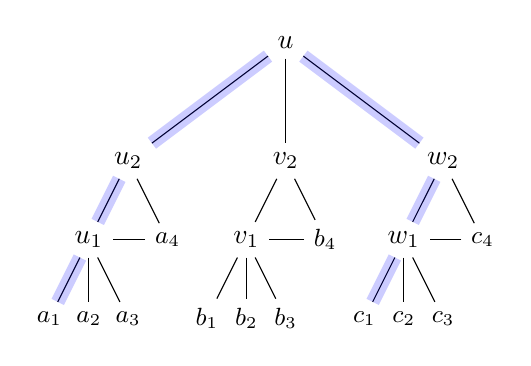
\begin{tikzpicture}
	\foreach \i/\a/\b in {0/a/u, 1/b/v, 2/c/w}{
		\node at (\i*2,0) (\a1) {\small$\a_1$};
		\node at (\i*2+0.5,0) (\a2) {\small$\a_2$};
		\node at (\i*2+1,0) (\a3) {\small$\a_3$};
		\node at (\i*2+0.5,1) (\b1) {$\b_1$} edge (\a1) edge (\a2) edge (\a3);
		\node at (\i*2+1.5,1) (\a4) {\small$\a_4$} edge (\b1);
		\node at (\i*2+1,2) (\b2) {$\b_2$} edge (\a4) edge (\b1);
	}
	\node at (3,3.5) (u) {$u$} edge (u2) edge (v2) edge (w2);
	\draw[color=blue,line width=5pt,opacity=0.2] (u1) edge (a1) (u2) edge (u1) (u) edge (u2) (u) edge (w2) (w2) edge (w1) (w1) edge (c1);
\end{tikzpicture}
\caption{\small Part of the hierarchy of the graph is shown on top. Edges of the same color have the same fraction and $\eps\gg \eta$ is a small constant. $u_1$ corresponds to the degree cut 
$\{a_1,a_2,a_3\}$, $u_2$ corresponds to the triangle cut $\{u_1,a_4\}$ and $u$ corresponds to the degree cut containing all of the vertices shown. Observe that edges in $\delta^\uparrow(a_1)$ are top edges in the degree cut $u$. 
If $\eps<\frac12 \eps_{1/1}$ then the $(A,B,C)$-degree partitioning
of edges in $\delta(u_2)$ is as follows: 
$A=\delta(a_1)\cap\delta(u_2)$ are the blue highlighted edges each of fractional value $1/2-\eps$, $B=\delta(a_4)\cap\delta(u_2)$ are the green highlighted edges of total fractional value 1, and $C$ are the red highlighted edges each of fractional value $\eps$. The cuts that contain edge $(a_1,c_1)$ are highlighted in the  hierarchy at the bottom.
}
\label{fig:topedgeABCmotivation}
\end{figure}

A few observations are  in order:
\begin{itemize}
\item Since $u$ is a candidate for, say $a$, it must be that $a$ is a descendent of $u$  in the hierarchy (or equal to $u$). In addition, $b$ cannot simultaneously be in $u$, since $a\cap b=\emptyset$ and $x(\delta(u) \cap\delta(u')) \le 1$ by \cref{lem:shared-edges}.  So, when $\bbf$ is 2-1-1 happy w.r.t.   $u'$ we get $(\delta(u)\cap\delta(u'))_T=1$.
\item If $u'=(X,Y)$ is a actual triangle cut, then we must have $a\subseteq X, b\subseteq Y$. So, when $\bbf$ is 2-1-1 happy w.r.t. $u'$, we know that $u'$ is a happy triangle, i.e., $(\delta(X)\cap\delta(u'))_T=1$ and $(\delta(Y)\cap\delta(u'))_T=1$.
\end{itemize}

Now, suppose for simplicity that all top edges in $\delta(u')$ are 2-1-1 good w.r.t. $u'$. Then, when an edge $g\in\delta(u)\cap\delta(u')$ is reduced, $(\delta(u)\cap\delta(u'))_T=1$, so 
$$ \P{\delta(u)_T\text{ odd} | g\text{ reduced}} \leq \P{E(u,u'\smallsetminus u)_T\text{ even}| g\text{ reduced}}\leq 0.57,$$
since edges in $E(u,u'\smallsetminus u)$ are in the tree independent of the reduction and $\E{E(u,u'\smallsetminus u)_T}\approx 1$.





%Our reduction rules will require that   given that an edge bundle $\bbe= (u',v')$ in $\delta (u) \cap \delta(u')$ is reduced, half of the time, it is 2-1-1- happy with respect to $u'$, i.e., $A_T$ and $B_T$ are odd, and $\delta(v')_T$ is even. When this happens, we can show that $(\delta(u) \smallsetminus  \delta (u'))_T$ is very likely to be odd, which suffices to show that $\P{\delta(u)_T\text{ odd} | \bbe\text{ reduced}}$ is only slightly more than 1/2. To complete the analysis, we show that at least a fraction 1/2 of the edges in $\delta^\uparrow (u)$ have constant probability of being  2-1-1 good in this more general sense. 

\paragraph{Dealing with $x_u$ close to 0 and the matching.}
\hypertarget{xu-close-to-zero}{We already} discussed how the matching is modified to handle the existence of bad edges. We now observe that we can handle the case $x_u \approx 0$ by further modifying the matching. 
The key observation is that  in this case, $x(\delta ^\rightarrow(u))\gg x(\delta ^\uparrow(u))$. Roughly speaking, this enables us to find a matching in which 
%$\sum_{\bbe \in \delta^\rightarrow(u)}m_{\bbe,u} = 2 x(\delta^\uparrow(u))$, so 
each edge in $\delta^\rightarrow(u)$ has to increase about half as much as would normally be expected to fix the cut of $u$. This eliminates the need to prove a nontrivial bound on $\P{\delta(u)_T\text{ odd} | g\text{ reduced}}$. The details of the matching are in \cref{sec:matching}.


%\vspace{0.1in}
%As a possible aid to the reader, we have collected much of the notation and some of the key helper lemmas in \cref{app:notation}.

%\paragraph{A note about the constants in our proof.}


